\section{Numerical results\label{sec:numres}}

In this section, numerical simulations are used to assess the
performance of the MFD solver in solving the quasi-static force-free
model (Equations~\eqref{eq:4.565}--\eqref{eq:4.580}) with different
configurations.  The simulations were carried out on NERSC's Cori and
Perlmutter machines.  For our computations on Cori, we used 4 Haswell
nodes for a total of 128 cpus.  For our computations on Perlmutter, we
used 1 CPU-only node for a total of 128 cpus.

% Cori is a Cray XC40 with a peak performance of about 30 petaflops and
%is comprised of 2388 Intel Xeon "Haswell" processor nodes and 9688
%Intel Xeon Phi "Knight's Landing" (KNL) nodes. 
%On Cori, the computations were carried out on Haswell Compute Nodes: Each node has two sockets, each
%socket is populated with a 2.3 GHz 16-core Haswell processor (Intel
%Xeon Processor E5-2698 v3). Each core supports 2 hyper-threads, and
%has two 256-bit-wide vector units. The theoretical peak is 36.8
%Gflops/core, 1.2 TFlops/node and 2.81 PFlops total. Each node has 128
%GB of DDR4 2133 MHz memory (four 16 GB DIMMs per socket) for a total
%aggregate memory of 298.5 TB. 

% Perlmutter is a Cray EX supercomputer comprising 3072 CPU-only and 1536 GPU-accelerated nodes and has a performance of 3-4 times Cori. 
%On Perlmutter, the computations were run on CPU-only nodes: each nodes is populated with two 2.45GHz 64-core AMD EPYC 7763 processors. 
%The theoretical peak is 39.2 Gflops/core, 2.52 TFlops/socket and 7.7 PFlops total. Each node has 512 GB of DDR4 memory for a total aggregate memory of 1536 TB. In our computations, we used 4 Haswell nodes for a total of 128 cpus.

% Talk about PETSc (references 34-36 can be found https://aip.scitation.org/doi/pdf/10.1063/1.2838244, and there are more referenes on PETSc's webpage)
For parallelization, we employ the Parallel Extensible Toolkit for
Scientific computing (PETSc) library \cite{petsc-web-page,
  petsc-user-ref, petsc-efficient}.
% Cite TS component of PETSc 
For the time-integration, we rely on PETSc's TS library that provides a framework for the scalable solvers of ODEs and DAEs arising from the discretization of time-dependent PDEs \cite{AbhyankarEtAl2018}.
%The list of available methods comprises, inter alia, IMEX Runge-Kutta schemes, Forward and Backward Euler, Crank-Nicolson,  Rosenbrock W-schemes and GL schemes with global error estimation.
The major data structure we build our MFD algorithm upon is DMStag~\cite{Sanan2022}, 
which is PETSc's distributed data structure for a full set of staggered grid representations. 
This allows the degrees of freedom to be associated with all ``strata'' in a logically-rectangular grid, i.e., elements, faces, edges, and vertices.
Note that such representations are more than the commonly used dual mesh setting
such as those in FDTD. 
We use a second-order L-stable DIRK time integrator and JFNK preconditioned by the finite difference coloring Jacobian.
Our major criterion for the solver convergence is the relative tolerance of the Newton iteration, which is always set as \num{1e-4}.
The linear solver tolerance is dynamically controlled by the inexact Newton algorithm,
 which  is used to reduce the total number of linear iterations. 

% Talk about the mesh resolution
All the simulations  presented in the current work are run on a cylindrical mesh that has a resolution of
$100 \times 2 \times 200$, i.e., 100 cells in $R$ direction, 2 cells with
periodic boundary conditions in $\phi$ direction and 200 cells in $Z$
direction. A minimal number of grid points in $\phi$ direction are used
since we only consider the axisymmetric case in this work.
However, we maintain a general implementation of full 3D operators, aiming for the whole device 
modeling capability and study of asymmetric cases in the future work.
% Cite DMStag component of PETSc


 The numerical results are organized into five sections. 
 Section~\ref{sec:resistivity} first investigates the impact of resistivity in the vacuum vessel.
 Since the model considered here misses a temperature equation (it will be considered as 
 the immediate follow-up work), the physically relevant resistivity value can be only determined numerically.
 We propose a simple approach to evaluate the model using the diffusion model in the vacuum vessel. 
 Section~\ref{sec:initial} then discusses the steps to prepare the initial condition. 
 As an exactly force-free magnetic field is known to be challenging to find, we propose
 a modeling approach to further reduce the $\j\times\B$ force. 
 The impact of different regularization terms are then studied in Section~\ref{sec:num_regularization}.
 The full VDE simulation is presented in Section~\ref{sec:vde}. 
 Finally, the study of the solver performance is presented in Section~\ref{sec:performance}. 

\subsection{Computing the effective resistivity of ITER vacuum vessel}
\label{sec:resistivity}

The ITER tokamak reactor has an interesting engineering design in
which the vacuum vessel (vv) is to carry the inductive toroidal current as
the response to a dynamically evolving plasma, such as that during a
VDE after a thermal quench.  To enable this, the blanket modules,
which are attached to the vacuum vessel and face the plasma, are
insulated from each other along the toroidal direction so no net
toroidal current is allowed in the blanket modules.  To model the
plasma VDE properly, one must properly account for the image current,
especially the toroidal one, in the vacuum vessel.  The actual ITER
vacuum vessel has complicated structures and a hollow interior for
neutron moderating inserts, the details of which are not necessary in
the usual plasma modeling. The essential property of the vacuum vessel
for plasma modeling is its characteristic time for a wall current to
decay in the absence of a plasma inside the chamber.  This so-called
wall time of the vacuum vessel, $\tau_{\rm vv} \equiv L/R,$ is the ratio
of inductance $L$ and resistance $R$ of the metal structure. The
inductance $L$ is set by the geometry of the conducting structure,
while $R$ has seperate toroidal and poloidal values, corresponding to
the decay of a net toroidal and a poloidal current in the vacuum
vessel. For wall feedback on VDEs, the toroidal one is most important,
and for ITER, the toroidal wall time is known to be around \SI{500}{\milli\second}. The
geometric simplification of the vaccum vessel, shown in light blue
(value of -1 for the levelset function) in Figure~\ref{fig:5layer},
implies that the correct $\tau_{\rm vv}=$~\SI{500}{\milli\second} can be recovered by an
effective electric resistivity $\eta_{\rm vv}$ for the vacuum vessel that
would be somewhat different from $\eta$ of the stainless steel
that is used to construct the vacuum vessel.  This effective
$\eta_{\rm vv}$ is directly computed here to match a given $\tau_{\rm vv}$ as
follows.

The goal here is to consider an isotropic vacuum vessel with uniform
resistivity, and find the resistivity value that would yield the
targeted wall time for ITER setting (around \SI{500}{\milli\second}). For that
purpose, we run initial stand-alone tests for the magnetic diffusion problem where
we take the same high resistivity value (to mimic a vacuum response)
for all the computational domain except the vacuum vessel, and a lower
resistivity value for the vacuum vessel $\Omega^{V}$. The initial
magnetic field has to be set such that the current is nonzero only in
the vacuum vessel. We recall that the magnetic field in the tokamak
can be represented by
\begin{equation}
{\B} = \nabla \phi \times \nabla \psi + g_0 \nabla \phi, 
\label{eqn:Bfrompsi}
\end{equation} 
where $\psi$ is the poloidal flux function and $g_0$ is a scalar constant. 

\begin{figure}[ht]
\begin{center}
%\includegraphics[width=\textwidth]{curlB.png}
\includegraphics[trim={10cm 0 1cm 0},clip, width=0.5\textwidth]{curlB.png}
\caption{The curl of the initial magnetic field in $\mathbf{e}_{\phi}$ direction.} 
\label{fig:5-layer_J0}
\end{center}
\end{figure} 

Enforcing a magnetic field such that the current is nonzero only in
the vacuum vessel amounts to solving the fixed-boundary Grad-Shafranov problem
\begin{equation}\label{eq:fixedbdeq}
  \begin{aligned}
    \frac{1}{\mu_0 R} ~ \Delta^{*} \psi & = J_0 && \text{in} \quad \Omega^{V}, \\
    \frac{1}{\mu_0 R} ~ \Delta^{*} \psi & = 0 && \text{in} \quad \Omega \setminus \Omega^{V}, \\
    \psi & = 0,&& \text{on} \quad \partial \Omega;
  \end{aligned}
\end{equation} 
where the toroidal elliptic operator is defined as   
\begin{equation*}
\Delta^* \psi := \dfrac{\partial^2 \psi}{\partial R^2}-\dfrac{1}{R}\dfrac{\partial \psi}{\partial R}+ \dfrac{\partial^2 \psi}{\partial Z^2},
\end{equation*}
After solving the problem~\eqref{eq:fixedbdeq}, and computing the
magnetic field with~\eqref{eqn:Bfrompsi}, we obtain the current shown
in Figure~\ref{fig:5-layer_J0}.

\begin{figure}[ht]
\centering
\begin{subfigure}[b]{0.5\textwidth}
\centering
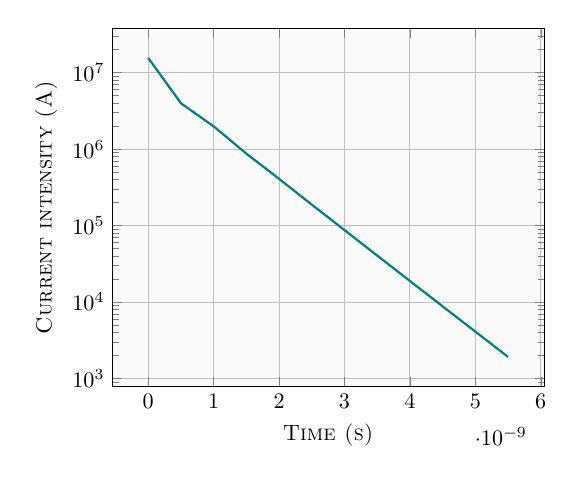
\begin{tikzpicture}[scale=.8,>=latex]
\begin{axis}[ymode=log, xlabel=\textsc{{Time (s)}}, ylabel=\textsc{{Current intensity (A)}}, ymajorgrids, xmajorgrids, axis background/.style={fill=gray!4},, legend style={legend columns=2,at={(0.5,-0.2)},anchor=north}]
\addplot+[color=teal,line width=1pt,mark=none] coordinates {(0, 1.55782e+07) (0.5e-9, 3.97973e+06) (1e-9, 1.9874e+06) (1.5e-9, 872492) (2e-9 , 408238) (2.5e-9, 187740) (3e-9, 87194.3) (3.5e-9, 40461.7) (4e-9, 18828.8) (4.5e-9, 8771.88) (5e-9, 4092.83) (5.5e-9, 1911.82)};
\end{axis}
\end{tikzpicture}
\caption{$\eta_{\rm vv} = 10^3 ~\SI{}{\ohm\meter}$}
\label{fig:current_vvdiffusion_S2e-2_2e-5_time}
\end{subfigure}%
~
\begin{subfigure}[b]{0.5\textwidth}
\centering
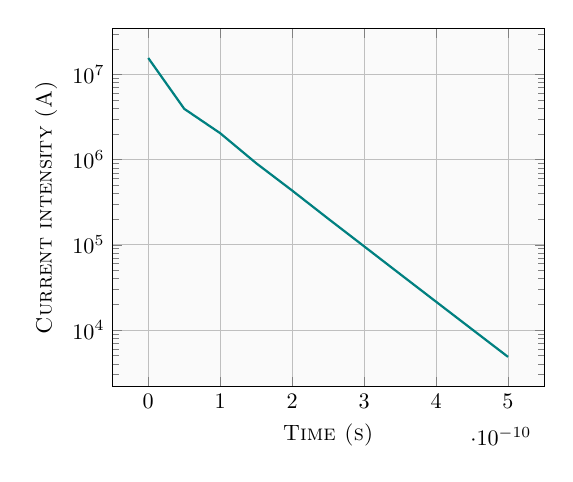
\begin{tikzpicture}[scale=.8,>=latex]
\begin{axis}[ymode=log, xlabel=\textsc{{Time (s)}}, ylabel=\textsc{{Current intensity (A)}}, ymajorgrids, xmajorgrids, axis background/.style={fill=gray!4},, legend style={legend columns=2,at={(0.5,-0.2)},anchor=north}]
\addplot+[color=teal,line width=1pt,mark=none] coordinates {(0, 1.55782e+07) (5.0e-11, 3.94512e+06) (1e-10, 2.0403e+06) (1.5e-10, 906796) (2e-10 , 433197) (2.5e-10, 202728) (3e-10, 95922.9) (3.5e-10, 45317.9) (4e-10, 21472.3) (4.5e-10, 10183.3) (5e-10, 4836.51)};
\end{axis}
\end{tikzpicture}
\caption{$\eta_{\rm vv} = 10^4 ~\SI{}{\ohm\meter}$}
\label{fig:current_vvdiffusion_S2e-3_2e-5_time}
\end{subfigure}     
\caption{Evolution of the current intensity inside the vacuum vessel over time with two different vacuum vessel resistivities $\eta_{\rm vv}$ and a fixed resistivity elsewhere $\eta= 10^6 ~\SI{}{\ohm\meter}$.}   
\end{figure}

Then, the diffusion model (Equations~\eqref{eq:4.572}--~\eqref{eq:4.576}) is solved.
With a resistivity value of $\eta_{\rm vv} = \SI{1e+3}{\ohm\meter}$
(i.e., a Lundquist number $S_{\rm vv} = \num{2.7646e-2}$ if the resistive diffusion time is normalized by the plasma Alfven time) inside the
vacuum vessel and $\eta = \SI{1e+6}{\ohm\meter}$ ($S =
\num{2.7646e-5}$) elsewhere, we obtain the current evolution depicted
in Figure~\ref{fig:current_vvdiffusion_S2e-2_2e-5_time}.  The slope is estimated as
%at $t=0$ is equal to:
\begin{equation*}
a_1 := \dfrac{\ln(10^5) - \ln(10^6)}{\num{3e-9} - \num{1.5e-9}} = \SI{-1.53e+9}{\second^{-1}}.
\end{equation*}


With a resistivity value of $\eta_{\rm vv} = \SI{1e+4}{\ohm\meter}$ (i.e., a Lundquist number $S_{\rm vv} = \num{2.7646e-3}$) inside the vacuum vessel and $\eta = \SI{1e+6}{\ohm\meter}$ ($S = \num{2.7646e-5}$) elsewhere, we obtain the current evolution depicted in Figure~\ref{fig:current_vvdiffusion_S2e-3_2e-5_time}. 
The slope %at $t=0$ 
is now equal to:
\begin{equation*}
a_2 := \dfrac{\ln(10^5) - \ln(10^6)}{\num{3e-10} - \num{1.5e-10}} = -\SI{1.53e+10}{\second^{-1}}.
\end{equation*}

\begin{figure}[ht]
\centering
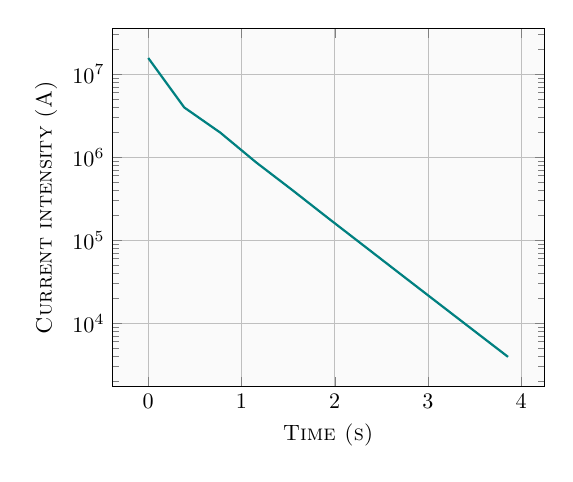
\begin{tikzpicture}[scale=.8,>=latex]
\begin{axis}[ymode=log, xlabel=\textsc{{Time (s)}}, ylabel=\textsc{{Current intensity (A)}}, ymajorgrids, xmajorgrids, axis background/.style={fill=gray!4},, legend style={legend columns=2,at={(0.5,-0.2)},anchor=north}]
\addplot+[color=teal,line width=1pt,mark=none] coordinates {(0, 1.55781e+07) (0.3858, 3.95356e+06) (0.771606, 1.97043e+06) (1.157409, 860919) (1.543212 , 401278) (1.929015, 183727) (2.314818, 84977.2) (2.700621, 39265.7) (3.086424, 18195.9) (3.472227, 8441.54) (3.858030, 3922.26)};
\end{axis}
\end{tikzpicture}
\caption{Evolution of the current intensity inside the vacuum vessel over time with $\eta_{\rm vv} = \SI{1.30288e-6}{\ohm\meter}$.}
\label{fig:current_vvdiffusion_S2e+7_2e+4_time}
\end{figure}

The characteristic time scale $L/R$ or wall time is expressed as
\begin{equation*}
\tau_{\rm vv} = \dfrac{L}{R_t},
\end{equation*}
with $L$ the inductance and the toroidal resistance
\begin{equation*}
R_t = \dfrac{2 \pi R \eta}{\mathcal{A}};
\end{equation*}
 $\mathcal{A}$ being the cross section.
The current decay is such that 
\begin{equation*}
I(t) = I_0 \exp(-\dfrac{t}{\tau_{\rm vv}}).
\end{equation*}
With the slopes computed previously, we can deduce that the resistivity value corresponding to $\tau_{\rm vv} = \SI{500}{\milli\second}$ is: 
\begin{equation}
\eta_{\rm vv} = \SI{1.30288e-6}{\ohm\meter} .
\label{eqn:vvresistivity}
\end{equation}
\noindent With such a resistivity ($S_{\rm vv} = 21219200$) inside the vacuum vessel and $\eta = \SI{1.30288e-3}{\ohm\meter}$ ($S = 21219.2$) elsewhere, we obtain the current evolution depicted in Figure~\ref{fig:current_vvdiffusion_S2e+7_2e+4_time}. 
The slope %at $t=0$ 
is equal to:
\begin{equation*}
a_3 := \dfrac{\ln(3922.26) - \ln(860919)}{3.858030 - 1.157409} = \SI{-1.99633062361}{\second^{-1}},
\end{equation*} 
which is very close to the expected value $\dfrac{-1}{\tau_{\rm vv}} = \dfrac{-1}{0.5} = \SI{-2}{\second^{-1}}$.



